%%%%%%%%%%%%%%%%%%%%%%%%%%%%%%%%%%%%%%%%%%%%%%%%%%%%%%%%%%%%%%%%%%%%%%%%%%%%%%%%%%%%%
\section{Conclusions}\label{sec:conclusions}
%%%%%%%%%%%%%%%%%%%%%%%%%%%%%%%%%%%%%%%%%%%%%%%%%%%%%%%%%%%%%%%%%%%%%%%%%%%%%%%%%%%%%

\todo{Chat GPT the shit of everything below}
In this work, three analyses were performed with data from the HAWC and IceCube observatories in order to explore some of the fundamental questions in particle astrophysics.
Thegoal was to contribute to the understanding of the sources of cosmic rays, their acceleration mechanisms, and the nature of dark matter. The detection techniques and reconstruction methods for both observatories were described, along with the properties that make them ideal instruments to perform such searches.

This dissertation used data from the HAWC detector to probe cutting-edge physics beyond the Standard Model.
The techniques by which HAWC is able to detect cosmic gamma rays were
demonstrated and the many advantages of HAWC in probing ultra-high energy gamma-ray physics were detailed.
It was shown how HAWC data can be used to explore unanswered questions such as the nature of dark matter and the limits of Lorentz invariance.
In particular, a search for evidence of WIMP dark matter in the Milky Way Galactic Halo was performed.
To accomplish this, simulations of the dark matter density profile were combined with estimates of the HAWC sensitivity to dark matter-like energy spectra.
This allowed strong constraints on dark matter annihilation and decay from the Galactic Halo to be derived that are insensitive to the large uncertainties arising from systematics in the dark matter spatial distribution.
Multi-hundred TeV photon spectra were also significantly detected from HAWC sources within the Galactic Plane. These results lead to the strongest constraints on Lorentz invariance violation to be published at the time of writing.

The work of this dissertation was made possible by the ongoing development of new algorithms and reconstruction techniques within the HAWC collaboration.
Probing the Galactic Halo required the creation of a novel background estimation technique that relied on HAWC’s wide field of view and strong ability to discriminate between gamma rays and cosmic rays.
Meanwhile, the constraints on Lorentz invariance violation were enabled by the improved energy resolution from a machine learning technique.
HAWC has recently completed a reprocessing of all archival data using an updated set of algorithms that can lead to compelling follow-up work on these results.
Combining the new background technique with the re-optimized energy estimators will allow for Galactic dark matter to be probed at even higher masses, as well as for analyses that require precise energy resolution such as gamma-ray line searches.

%%%%%%%%%%%%%%%%%%%%%%%%%%%%%%%%%%%%%%%%%%%%%%%%%%%%%%%%%%%%%%%%%%%%%%%%%%%%%%%%%%%%%
\section{Future Directions: Multi-Messenger Dark Matter Search}\label{sec:future}
%%%%%%%%%%%%%%%%%%%%%%%%%%%%%%%%%%%%%%%%%%%%%%%%%%%%%%%%%%%%%%%%%%%%%%%%%%%%%%%%%%%%%

\begin{figure}[h]
    \centering{
        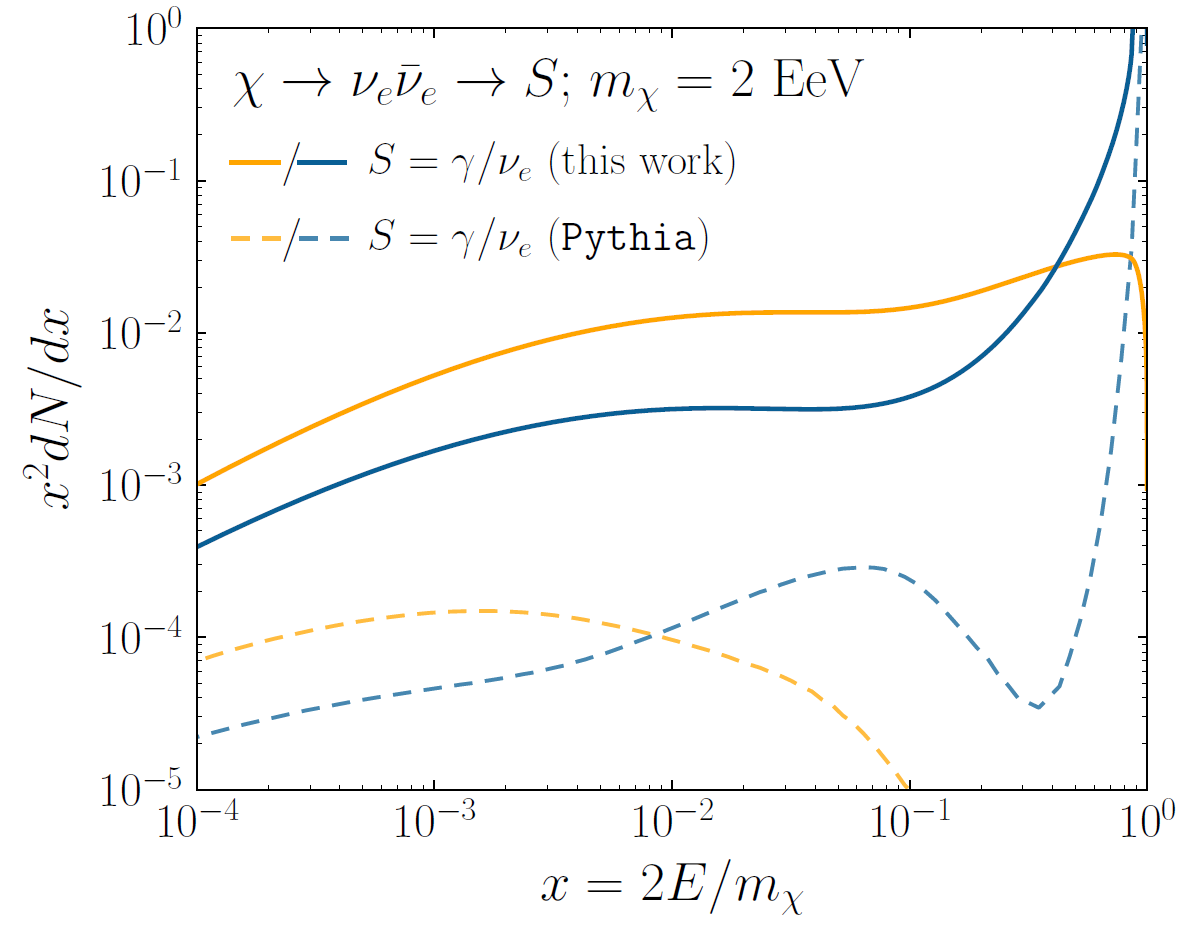
\includegraphics[scale=0.4]{figures/hdm_gamma_nu.png}
    }
    \caption{The prompt electron neutrino and photon spectrum resulting from the decay of a 2EeV DM particle to \parpar{\nu_e}, as currently being searched for at IceCube [5]. Solid curves represent the results of this work, and predict orders of magnitude more flux at certain energies than the dashed results of Pythia 8.2, one of the only existing methods to generate spectra at these masses. In both cases energy conservation is satisfied: there is a considerable contribution to a $\delta$-function at x = 1, associated with events where an initial W or Z was never emitted and thus no subsequent shower developed. Large disagreements are generically observed at these masses for electroweak dominated channels, while the agreement is better for colored initial SM states.}
    \label{fig:nu_and_gam}
\end{figure}

As I have shown previously in \cref{sec:glory_duck} and \cref{sec:multithread}, we can build a fast and robust analysis that shares tools with the field.
The hope being that IceCube can eventually combine data with gamma-ray observatories.
\tmpfig{nuetrino and bb plot with nu Sensitivities}